\begin{block}{Problem Statement}
  Jordan has a credit limit of \$3,000 and carries an initial balance of \$600. He makes a new purchase of \$750 on the card.

  What is Jordan's new credit utilization ratio after this purchase?
\end{block}

\vspace{0.8em}
\centering
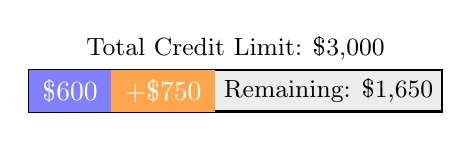
\begin{tikzpicture}[scale=0.75]
  \draw[thick, fill=gray!15] (0,0) rectangle (7,0.7);
  \fill[blue!50] (0,0) rectangle (1.4,0.7);
  \fill[orange!70] (1.4,0) rectangle (3.15,0.7);
  \node at (0.7,0.35) {\color{white}\$600};
  \node at (2.275,0.35) {\color{white}+\$750};
  \node at (5.075,0.35) {\small Remaining: \$1,650};
  \node[above] at (3.5,0.7) {\small Total Credit Limit: \$3,000};
\end{tikzpicture}
